\documentclass[11pt]{article}

\usepackage[margin=1in]{geometry}
\usepackage{graphicx}
\usepackage{array}
\usepackage{longtable}
\usepackage{hyperref}
\usepackage{booktabs}
\usepackage{xcolor}
\usepackage{tikz}
\usepackage{float}
\usepackage{enumitem}
\usepackage{fancyhdr}
\usepackage{titlesec}
\usepackage{tcolorbox}
\usepackage{tabularx}
\usepackage{multirow}
\usepackage{caption}
\usepackage{subcaption}
\usepackage{listings}
\usepackage{makecell}
\usepackage{pgfplots}
\pgfplotsset{compat=1.17}

\usetikzlibrary{shapes.geometric, arrows.meta, positioning, fit, backgrounds, calc, decorations.pathreplacing, shapes.multipart, matrix, shadows}

% Color definitions
\definecolor{componentcolor}{RGB}{70,130,180}
\definecolor{modulecolor}{RGB}{60,179,113}
\definecolor{servicecolor}{RGB}{255,165,0}
\definecolor{datacolor}{RGB}{186,85,211}
\definecolor{flowcolor}{RGB}{100,100,100}
\definecolor{sectionblue}{RGB}{31,78,121}
\definecolor{lightgray}{RGB}{245,245,245}
\definecolor{warningred}{RGB}{220,53,69}
\definecolor{successgreen}{RGB}{40,167,69}
\definecolor{infoblue}{RGB}{23,162,184}
\definecolor{layercolor1}{RGB}{173,216,230}
\definecolor{layercolor2}{RGB}{144,238,144}
\definecolor{layercolor3}{RGB}{255,218,185}
\definecolor{layercolor4}{RGB}{221,160,221}
\definecolor{connectorcolor}{RGB}{255,99,71}
\definecolor{portcolor}{RGB}{255,215,0}

% Hyperref setup
\hypersetup{
    colorlinks=true,
    linkcolor=sectionblue,
    urlcolor=sectionblue,
    citecolor=sectionblue
}

% Header and footer
\pagestyle{fancy}
\fancyhf{}
\fancyhead[L]{\leftmark}
\fancyhead[R]{Primary Presentation Documentation}
\fancyfoot[C]{\thepage}
\renewcommand{\headrulewidth}{0.4pt}
\renewcommand{\footrulewidth}{0.4pt}

% Section formatting
\titleformat{\section}
  {\normalfont\Large\bfseries\color{sectionblue}}{\thesection}{1em}{}
\titleformat{\subsection}
  {\normalfont\large\bfseries\color{sectionblue!80}}{\thesubsection}{1em}{}
\titleformat{\subsubsection}
  {\normalfont\normalsize\bfseries\color{sectionblue!60}}{\thesubsubsection}{1em}{}

% Custom box environments
\newtcolorbox{keypoint}{
    colback=blue!5,
    colframe=sectionblue,
    title=Key Point,
    fonttitle=\bfseries
}

\newtcolorbox{warning}{
    colback=red!5,
    colframe=warningred,
    title=Warning,
    fonttitle=\bfseries
}

\newtcolorbox{bestpractice}{
    colback=green!5,
    colframe=successgreen,
    title=Best Practice,
    fonttitle=\bfseries
}

\newtcolorbox{example}{
    colback=lightgray,
    colframe=flowcolor,
    title=Example,
    fonttitle=\bfseries
}

\newtcolorbox{definition}{
    colback=infoblue!10,
    colframe=infoblue,
    title=Definition,
    fonttitle=\bfseries
}

\newtcolorbox{template}{
    colback=white,
    colframe=flowcolor,
    title=Template,
    fonttitle=\bfseries
}

\newtcolorbox{designprinciple}{
    colback=servicecolor!10,
    colframe=servicecolor,
    title=Design Principle,
    fonttitle=\bfseries
}

% Code listing style
\lstset{
    basicstyle=\ttfamily\small,
    breaklines=true,
    frame=single,
    backgroundcolor=\color{lightgray},
    keywordstyle=\color{sectionblue},
    commentstyle=\color{successgreen},
    stringstyle=\color{servicecolor}
}

% Custom column types
\newcolumntype{L}[1]{>{\raggedright\arraybackslash}p{#1}}
\newcolumntype{C}[1]{>{\centering\arraybackslash}p{#1}}
\newcolumntype{R}[1]{>{\raggedleft\arraybackslash}p{#1}}

\title{%
    \vspace{-1cm}
    \textbf{\Huge Software Architecture Documentation}\\[12pt]
    \Large Primary Presentation\\[8pt]
    \large A Comprehensive Guide to Creating Effective\\
    Architectural Diagrams and Visual Documentation
}
\author{%
    \textit{Architecture Documentation Series}\\[4pt]
    \small Based on SEI Views and Beyond, C4 Model, UML, and Industry Best Practices
}
\date{\today}

\begin{document}

\maketitle
\thispagestyle{empty}

\vspace{0.8cm}

\begin{abstract}
\noindent
The Primary Presentation is the visual centerpiece of an architectural view---the diagram or set of diagrams that communicates the essential structure of a system at a glance. Effective primary presentations enable stakeholders to quickly grasp architectural decisions, understand system organization, and reason about quality attributes. This comprehensive guide establishes principles and best practices for creating primary presentations that are clear, accurate, informative, and maintainable. The document covers view type selection, diagram design principles, notation standards (UML, C4, ArchiMate, and custom notations), element representation, narrative techniques, behavioral integration, and governance processes. Whether documenting module structures, component-and-connector relationships, deployment topologies, or data flows, this guide provides the foundation for professional architectural visualization.
\end{abstract}

\vfill

\begin{center}
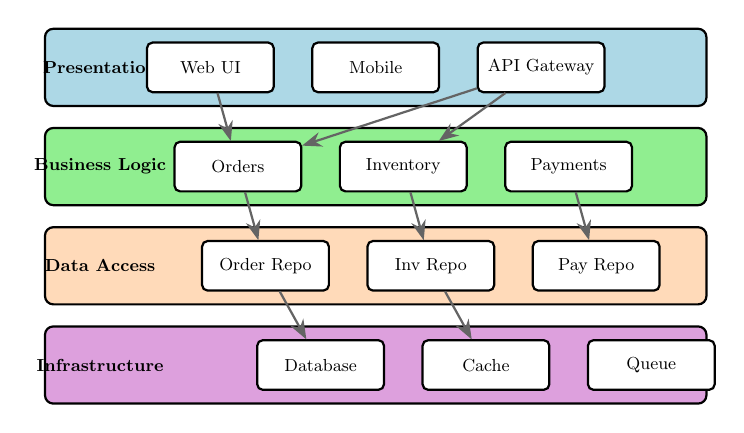
\begin{tikzpicture}[
    scale=0.7,
    transform shape,
    layer/.style={draw, thick, minimum width=12cm, minimum height=1.4cm, rounded corners=3pt},
    component/.style={draw, thick, fill=white, minimum width=2.3cm, minimum height=0.9cm, rounded corners=2pt, font=\small},
    arrow/.style={-{Stealth[length=2.5mm]}, thick, flowcolor}
]
    % Layers
    \node[layer, fill=layercolor1] (presentation) at (0,3) {};
    \node[layer, fill=layercolor2] (business) at (0,1.2) {};
    \node[layer, fill=layercolor3] (data) at (0,-0.6) {};
    \node[layer, fill=layercolor4] (infrastructure) at (0,-2.4) {};
    
    % Layer labels
    \node[font=\small\bfseries] at (-5,3) {Presentation};
    \node[font=\small\bfseries] at (-5,1.2) {Business Logic};
    \node[font=\small\bfseries] at (-5,-0.6) {Data Access};
    \node[font=\small\bfseries] at (-5,-2.4) {Infrastructure};
    
    % Components in Presentation
    \node[component] (web) at (-3,3) {Web UI};
    \node[component] (mobile) at (0,3) {Mobile};
    \node[component] (api) at (3,3) {API Gateway};
    
    % Components in Business
    \node[component] (orders) at (-2.5,1.2) {Orders};
    \node[component] (inventory) at (0.5,1.2) {Inventory};
    \node[component] (payments) at (3.5,1.2) {Payments};
    
    % Components in Data
    \node[component] (orderrepo) at (-2,-0.6) {Order Repo};
    \node[component] (invrepo) at (1,-0.6) {Inv Repo};
    \node[component] (payrepo) at (4,-0.6) {Pay Repo};
    
    % Components in Infrastructure
    \node[component] (db) at (-1,-2.4) {Database};
    \node[component] (cache) at (2,-2.4) {Cache};
    \node[component] (queue) at (5,-2.4) {Queue};
    
    % Arrows
    \draw[arrow] (web) -- (orders);
    \draw[arrow] (api) -- (orders);
    \draw[arrow] (api) -- (inventory);
    \draw[arrow] (orders) -- (orderrepo);
    \draw[arrow] (inventory) -- (invrepo);
    \draw[arrow] (payments) -- (payrepo);
    \draw[arrow] (orderrepo) -- (db);
    \draw[arrow] (invrepo) -- (cache);
\end{tikzpicture}
\end{center}

\newpage
\tableofcontents
\newpage

%==============================================================================
\section{Introduction to the Primary Presentation}
%==============================================================================

\subsection{Definition and Purpose}

The Primary Presentation is the principal graphical representation of an architectural view. It is the diagram (or coordinated set of diagrams) that shows, at a glance, the elements and relationships that constitute the architecture from a particular perspective. While supporting documentation provides detail, the primary presentation provides orientation and overview.

\begin{definition}
A \textbf{Primary Presentation} is the graphical depiction of an architectural view's elements and their relationships, designed to communicate the essential structure of the system to stakeholders in a form that can be quickly comprehended and reasoned about.
\end{definition}

The primary presentation serves several critical functions. First, it provides \textbf{orientation} by giving stakeholders a mental map of the system's structure. Second, it enables \textbf{communication} as a shared visual language for discussing architecture among diverse stakeholders. Third, it supports \textbf{analysis} by making structural patterns, dependencies, and potential issues visible. Fourth, it acts as \textbf{navigation} by providing an index to more detailed documentation. Fifth, it serves \textbf{decision support} by making architectural tradeoffs and alternatives visible.

\subsection{The Role Within Architectural Documentation}

Every architectural view consists of three complementary parts: the primary presentation (diagrams), the element catalog (detailed specifications), and the context documentation (rationale and background). The primary presentation is not the complete documentation---it is the visual summary that makes the detailed documentation accessible.

\begin{figure}[H]
\centering
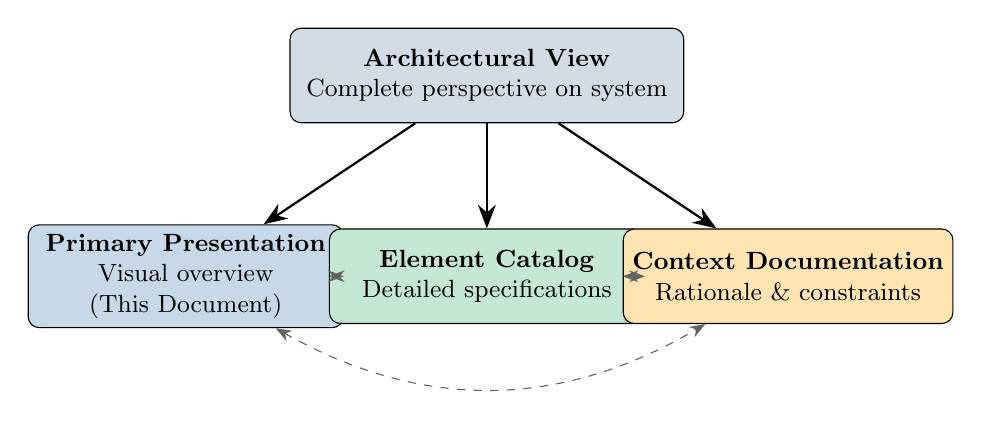
\begin{tikzpicture}[
    scale=0.85,
    box/.style={draw, rounded corners, minimum width=4cm, minimum height=1.2cm, align=center, font=\small},
    arrow/.style={-{Stealth[length=3mm]}, thick}
]
    % Central view
    \node[box, fill=sectionblue!20, minimum width=5cm] (view) at (0,3) {\textbf{Architectural View}\\Complete perspective on system};
    
    % Three parts
    \node[box, fill=componentcolor!30] (primary) at (-4.5,0) {\textbf{Primary Presentation}\\Visual overview\\(This Document)};
    \node[box, fill=modulecolor!30] (catalog) at (0,0) {\textbf{Element Catalog}\\Detailed specifications};
    \node[box, fill=servicecolor!30] (context) at (4.5,0) {\textbf{Context Documentation}\\Rationale \& constraints};
    
    % Arrows
    \draw[arrow] (view) -- (primary);
    \draw[arrow] (view) -- (catalog);
    \draw[arrow] (view) -- (context);
    
    % Cross-references
    \draw[{Stealth[length=2mm]}-{Stealth[length=2mm]}, dashed, flowcolor] (primary) -- (catalog);
    \draw[{Stealth[length=2mm]}-{Stealth[length=2mm]}, dashed, flowcolor] (catalog) -- (context);
    \draw[{Stealth[length=2mm]}-{Stealth[length=2mm]}, dashed, flowcolor] (primary) to[bend right=30] (context);
\end{tikzpicture}
\caption{Primary Presentation within View Documentation Structure}
\end{figure}

\subsection{Characteristics of Effective Primary Presentations}

Effective primary presentations share common characteristics. They are \textbf{comprehensible}, meaning a knowledgeable stakeholder can understand the main structure within minutes, not hours. They are \textbf{accurate}, meaning the diagram faithfully represents the actual or intended architecture. They are \textbf{complete} (for their purpose), meaning all elements relevant to the view's concerns are shown. They are \textbf{consistent}, meaning notation is used uniformly throughout the diagram. They are \textbf{minimal}, meaning unnecessary detail is omitted to maintain clarity. They are \textbf{navigable}, meaning viewers can find their way to detailed information. They are \textbf{maintainable}, meaning the diagram can be updated as the architecture evolves.

\begin{keypoint}
The primary presentation should answer the question: ``What is the structure of this system from this perspective?'' It should not attempt to answer every question about the architecture---that is the role of the complete documentation set.
\end{keypoint}

\subsection{Standards and Frameworks}

Primary presentation practices draw from several standards and methodologies. The SEI Views and Beyond approach explicitly defines the primary presentation as the first part of every architectural view. UML (Unified Modeling Language) provides standard notation for many diagram types. The C4 Model offers a hierarchical approach to system visualization. ArchiMate provides enterprise architecture notation. SysML extends UML for systems engineering. IEEE 42010 establishes the framework for architectural viewpoints that presentations support.

%==============================================================================
\section{View Types and Their Primary Presentations}
%==============================================================================

\subsection{Understanding View Types}

Different architectural concerns require different types of views, each with appropriate primary presentation styles. The choice of view type determines what elements appear and how they should be visualized.

\begin{figure}[H]
\centering
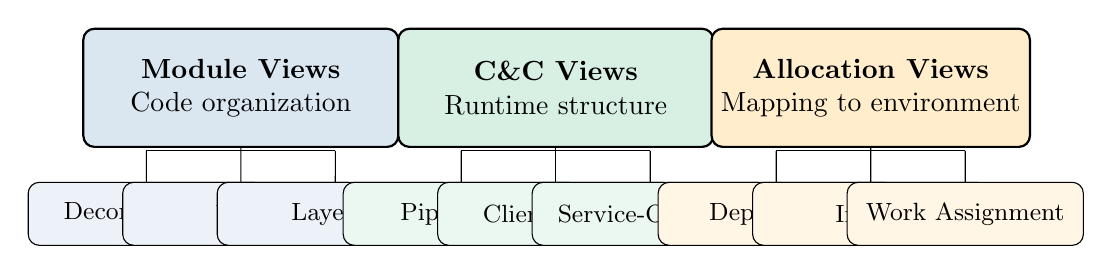
\begin{tikzpicture}[
    scale=0.8,
    category/.style={draw, thick, rounded corners, minimum width=4cm, minimum height=1.5cm, align=center},
    viewtype/.style={draw, rounded corners, minimum width=3cm, minimum height=0.8cm, align=center, font=\small}
]
    % Categories
    \node[category, fill=componentcolor!20] (module) at (-5,2) {\textbf{Module Views}\\Code organization};
    \node[category, fill=modulecolor!20] (cc) at (0,2) {\textbf{C\&C Views}\\Runtime structure};
    \node[category, fill=servicecolor!20] (alloc) at (5,2) {\textbf{Allocation Views}\\Mapping to environment};
    
    % View types under Module
    \node[viewtype, fill=componentcolor!10] (decomp) at (-6.5,0) {Decomposition};
    \node[viewtype, fill=componentcolor!10] (uses) at (-5,0) {Uses};
    \node[viewtype, fill=componentcolor!10] (layer) at (-3.5,0) {Layered};
    
    % View types under C&C
    \node[viewtype, fill=modulecolor!10] (pipe) at (-1.5,0) {Pipe-Filter};
    \node[viewtype, fill=modulecolor!10] (cs) at (0,0) {Client-Server};
    \node[viewtype, fill=modulecolor!10] (soa) at (1.5,0) {Service-Oriented};
    
    % View types under Allocation
    \node[viewtype, fill=servicecolor!10] (deploy) at (3.5,0) {Deployment};
    \node[viewtype, fill=servicecolor!10] (install) at (5,0) {Install};
    \node[viewtype, fill=servicecolor!10] (work) at (6.5,0) {Work Assignment};
    
    % Connections
    \draw[-] (module) -- (-5,1);
    \draw[-] (-6.5,1) -- (-3.5,1);
    \draw[-] (-6.5,1) -- (decomp);
    \draw[-] (-5,1) -- (uses);
    \draw[-] (-3.5,1) -- (layer);
    
    \draw[-] (cc) -- (0,1);
    \draw[-] (-1.5,1) -- (1.5,1);
    \draw[-] (-1.5,1) -- (pipe);
    \draw[-] (0,1) -- (cs);
    \draw[-] (1.5,1) -- (soa);
    
    \draw[-] (alloc) -- (5,1);
    \draw[-] (3.5,1) -- (6.5,1);
    \draw[-] (3.5,1) -- (deploy);
    \draw[-] (5,1) -- (install);
    \draw[-] (6.5,1) -- (work);
\end{tikzpicture}
\caption{Architectural View Type Categories}
\end{figure}

\subsection{Module Views}

Module views show the code-time structure of a system---how source code is organized into modules, packages, classes, and layers. Primary presentations for module views typically use box-and-line notation showing containment and dependency relationships.

\subsubsection{Module Decomposition View}

The decomposition view shows how the system is divided into modules and sub-modules. The primary presentation is typically a hierarchical diagram.

\begin{figure}[H]
\centering
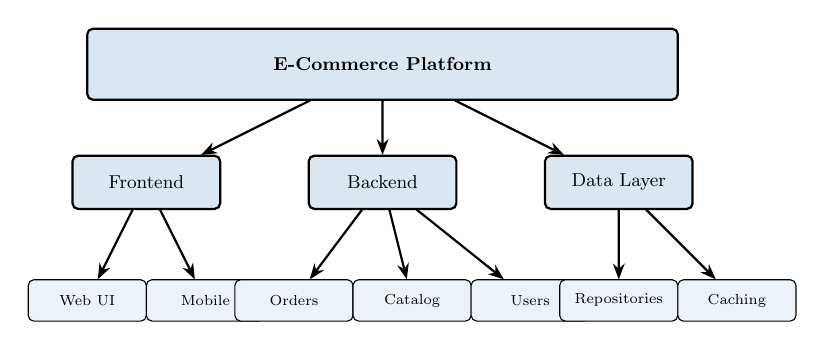
\begin{tikzpicture}[
    scale=0.75,
    transform shape,
    module/.style={draw, thick, fill=componentcolor!20, minimum width=2.5cm, minimum height=0.9cm, rounded corners=2pt, font=\small},
    submodule/.style={draw, fill=componentcolor!10, minimum width=2cm, minimum height=0.7cm, rounded corners=2pt, font=\scriptsize},
    contains/.style={-{Stealth[length=2mm]}, thick}
]
    % Top level
    \node[module, minimum width=10cm, minimum height=1.2cm] (system) at (0,4) {\textbf{E-Commerce Platform}};
    
    % Second level
    \node[module] (frontend) at (-4,2) {Frontend};
    \node[module] (backend) at (0,2) {Backend};
    \node[module] (data) at (4,2) {Data Layer};
    
    % Third level - Frontend
    \node[submodule] (web) at (-5,0) {Web UI};
    \node[submodule] (mobile) at (-3,0) {Mobile};
    
    % Third level - Backend
    \node[submodule] (orders) at (-1.5,0) {Orders};
    \node[submodule] (catalog) at (0.5,0) {Catalog};
    \node[submodule] (users) at (2.5,0) {Users};
    
    % Third level - Data
    \node[submodule] (repos) at (4,0) {Repositories};
    \node[submodule] (cache) at (6,0) {Caching};
    
    % Containment lines
    \draw[contains] (system) -- (frontend);
    \draw[contains] (system) -- (backend);
    \draw[contains] (system) -- (data);
    
    \draw[contains] (frontend) -- (web);
    \draw[contains] (frontend) -- (mobile);
    
    \draw[contains] (backend) -- (orders);
    \draw[contains] (backend) -- (catalog);
    \draw[contains] (backend) -- (users);
    
    \draw[contains] (data) -- (repos);
    \draw[contains] (data) -- (cache);
\end{tikzpicture}
\caption{Module Decomposition View Example}
\end{figure}

\subsubsection{Layered View}

The layered view organizes modules into layers with constrained dependencies (typically, a layer may only use the layer immediately below it). The primary presentation emphasizes the layer structure and allowed relationships.

\begin{figure}[H]
\centering
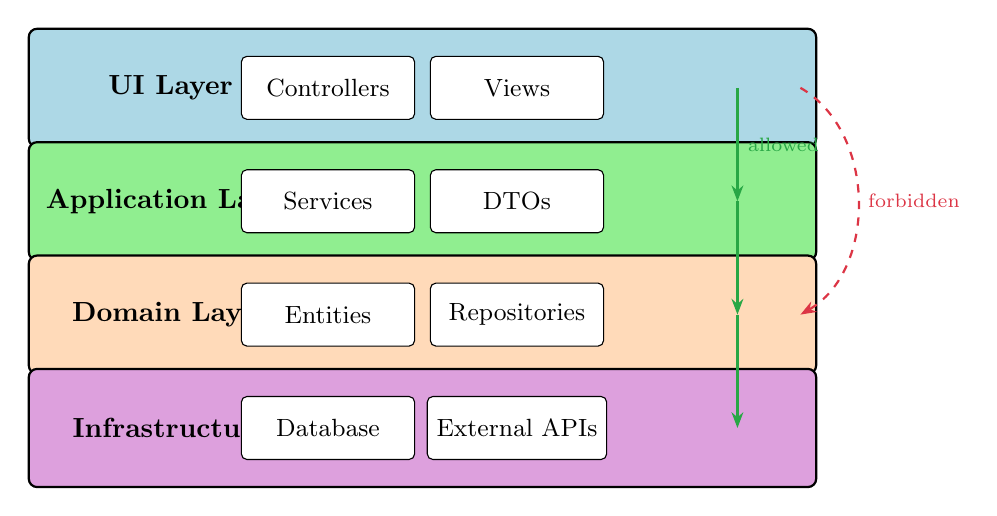
\begin{tikzpicture}[
    scale=0.8,
    layer/.style={draw, thick, minimum width=10cm, minimum height=1.5cm, rounded corners=3pt},
    module/.style={draw, fill=white, minimum width=2.2cm, minimum height=0.8cm, rounded corners=2pt, font=\small},
    allowed/.style={-{Stealth[length=2mm]}, thick, successgreen},
    forbidden/.style={-{Stealth[length=2mm]}, thick, warningred, dashed}
]
    % Layers
    \node[layer, fill=layercolor1] (ui) at (0,4.5) {};
    \node[layer, fill=layercolor2] (app) at (0,2.7) {};
    \node[layer, fill=layercolor3] (domain) at (0,0.9) {};
    \node[layer, fill=layercolor4] (infra) at (0,-0.9) {};
    
    % Layer labels
    \node[font=\bfseries] at (-4,4.5) {UI Layer};
    \node[font=\bfseries] at (-4,2.7) {Application Layer};
    \node[font=\bfseries] at (-4,0.9) {Domain Layer};
    \node[font=\bfseries] at (-4,-0.9) {Infrastructure};
    
    % Modules
    \node[module] at (-1.5,4.5) {Controllers};
    \node[module] at (1.5,4.5) {Views};
    
    \node[module] at (-1.5,2.7) {Services};
    \node[module] at (1.5,2.7) {DTOs};
    
    \node[module] at (-1.5,0.9) {Entities};
    \node[module] at (1.5,0.9) {Repositories};
    
    \node[module] at (-1.5,-0.9) {Database};
    \node[module] at (1.5,-0.9) {External APIs};
    
    % Dependency arrows (right side)
    \draw[allowed] (5,4.5) -- node[right, font=\scriptsize] {allowed} (5,2.7);
    \draw[allowed] (5,2.7) -- (5,0.9);
    \draw[allowed] (5,0.9) -- (5,-0.9);
    
    % Forbidden arrow
    \draw[forbidden] (6,4.5) to[bend left=60] node[right, font=\scriptsize] {forbidden} (6,0.9);
\end{tikzpicture}
\caption{Layered View with Dependency Rules}
\end{figure}

\subsubsection{Uses View}

The uses view shows which modules use (depend on) which other modules. The primary presentation is typically a directed graph.

\subsection{Component-and-Connector (C\&C) Views}

C\&C views show the runtime structure of a system---processes, threads, services, and the connectors through which they interact. Primary presentations for C\&C views emphasize components, their ports, and the connectors between them.

\subsubsection{Service-Oriented View}

\begin{figure}[H]
\centering
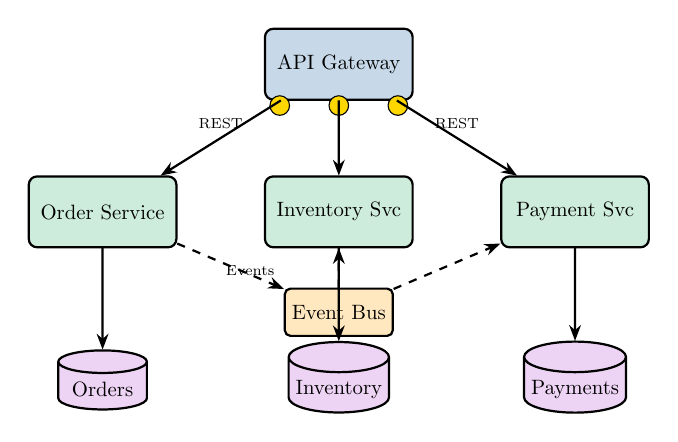
\begin{tikzpicture}[
    scale=0.75,
    transform shape,
    service/.style={draw, thick, fill=modulecolor!25, minimum width=2.5cm, minimum height=1.2cm, rounded corners=3pt},
    database/.style={draw, thick, fill=datacolor!25, cylinder, shape border rotate=90, aspect=0.3, minimum width=1.5cm, minimum height=1cm},
    queue/.style={draw, thick, fill=servicecolor!25, minimum width=1.8cm, minimum height=0.8cm, rounded corners=2pt},
    port/.style={draw, fill=portcolor, circle, minimum size=0.3cm},
    connector/.style={-{Stealth[length=2mm]}, thick},
    async/.style={-{Stealth[length=2mm]}, thick, dashed}
]
    % API Gateway
    \node[service, fill=componentcolor!30] (gateway) at (0,4) {API Gateway};
    
    % Services
    \node[service] (order) at (-4,1.5) {Order Service};
    \node[service] (inventory) at (0,1.5) {Inventory Svc};
    \node[service] (payment) at (4,1.5) {Payment Svc};
    
    % Databases
    \node[database] (orderdb) at (-4,-1.5) {Orders};
    \node[database] (invdb) at (0,-1.5) {Inventory};
    \node[database] (paydb) at (4,-1.5) {Payments};
    
    % Message Queue
    \node[queue] (events) at (0,-0.2) {Event Bus};
    
    % Ports on gateway
    \node[port] (gp1) at (-1,3.3) {};
    \node[port] (gp2) at (0,3.3) {};
    \node[port] (gp3) at (1,3.3) {};
    
    % Connectors
    \draw[connector] (gateway) -- (order);
    \draw[connector] (gateway) -- (inventory);
    \draw[connector] (gateway) -- (payment);
    
    \draw[connector] (order) -- (orderdb);
    \draw[connector] (inventory) -- (invdb);
    \draw[connector] (payment) -- (paydb);
    
    \draw[async] (order) -- (events);
    \draw[async] (events) -- (inventory);
    \draw[async] (events) -- (payment);
    
    % Labels
    \node[font=\scriptsize] at (-2,3) {REST};
    \node[font=\scriptsize] at (2,3) {REST};
    \node[font=\scriptsize] at (-1.5,0.5) {Events};
\end{tikzpicture}
\caption{Service-Oriented Architecture View}
\end{figure}

\subsubsection{Pipe-and-Filter View}

The pipe-and-filter view shows data processing pipelines where filters transform data and pipes transport it between filters.

\begin{figure}[H]
\centering
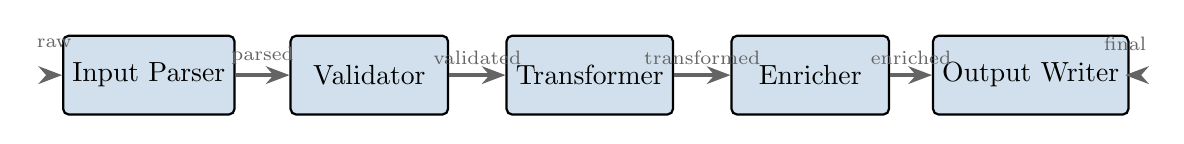
\begin{tikzpicture}[
    scale=0.8,
    filter/.style={draw, thick, fill=componentcolor!25, minimum width=2cm, minimum height=1cm, rounded corners=2pt},
    pipe/.style={-{Stealth[length=3mm]}, very thick, flowcolor},
    data/.style={font=\scriptsize, flowcolor}
]
    % Filters
    \node[filter] (input) at (0,0) {Input Parser};
    \node[filter] (validate) at (3.5,0) {Validator};
    \node[filter] (transform) at (7,0) {Transformer};
    \node[filter] (enrich) at (10.5,0) {Enricher};
    \node[filter] (output) at (14,0) {Output Writer};
    
    % Pipes
    \draw[pipe] (-1.5,0) -- (input);
    \draw[pipe] (input) -- node[above, data] {parsed} (validate);
    \draw[pipe] (validate) -- node[above, data] {validated} (transform);
    \draw[pipe] (transform) -- node[above, data] {transformed} (enrich);
    \draw[pipe] (enrich) -- node[above, data] {enriched} (output);
    \draw[pipe] (output) -- (15.5,0);
    
    % Data annotations
    \node[data] at (-1.5,0.5) {raw};
    \node[data] at (15.5,0.5) {final};
\end{tikzpicture}
\caption{Pipe-and-Filter View}
\end{figure}

\subsection{Allocation Views}

Allocation views show how software elements map to non-software elements in the environment---hardware, file systems, teams, and so forth.

\subsubsection{Deployment View}

The deployment view shows how software artifacts are deployed to hardware or virtualized infrastructure.

\begin{figure}[H]
\centering
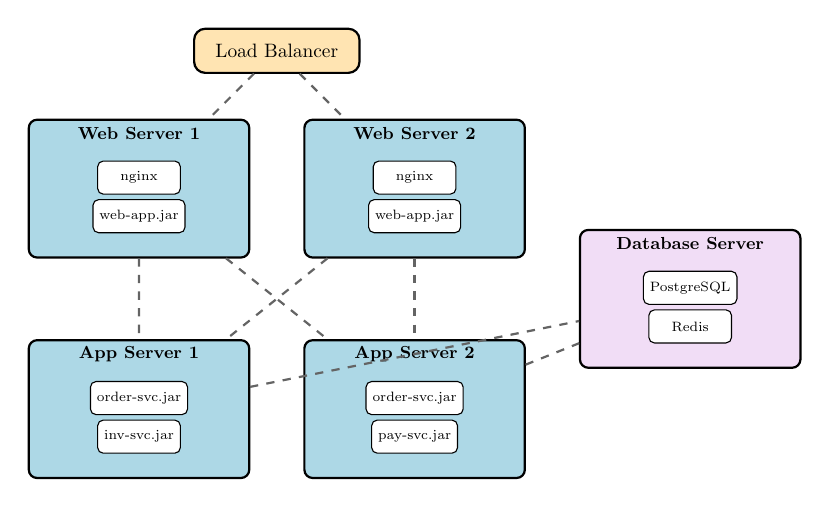
\begin{tikzpicture}[
    scale=0.7,
    transform shape,
    node/.style={draw, thick, fill=layercolor1, minimum width=4cm, minimum height=2.5cm, rounded corners=3pt},
    artifact/.style={draw, fill=white, minimum width=1.5cm, minimum height=0.6cm, rounded corners=2pt, font=\scriptsize},
    network/.style={draw, thick, dashed, flowcolor}
]
    % Nodes
    \node[node] (web1) at (-5,3) {};
    \node[font=\small\bfseries] at (-5,4) {Web Server 1};
    \node[artifact] at (-5,3.2) {nginx};
    \node[artifact] at (-5,2.5) {web-app.jar};
    
    \node[node] (web2) at (0,3) {};
    \node[font=\small\bfseries] at (0,4) {Web Server 2};
    \node[artifact] at (0,3.2) {nginx};
    \node[artifact] at (0,2.5) {web-app.jar};
    
    \node[node] (app1) at (-5,-1) {};
    \node[font=\small\bfseries] at (-5,0) {App Server 1};
    \node[artifact] at (-5,-0.8) {order-svc.jar};
    \node[artifact] at (-5,-1.5) {inv-svc.jar};
    
    \node[node] (app2) at (0,-1) {};
    \node[font=\small\bfseries] at (0,0) {App Server 2};
    \node[artifact] at (0,-0.8) {order-svc.jar};
    \node[artifact] at (0,-1.5) {pay-svc.jar};
    
    \node[node, fill=datacolor!20] (db) at (5,1) {};
    \node[font=\small\bfseries] at (5,2) {Database Server};
    \node[artifact] at (5,1.2) {PostgreSQL};
    \node[artifact] at (5,0.5) {Redis};
    
    % Network connections
    \draw[network] (web1) -- (app1);
    \draw[network] (web1) -- (app2);
    \draw[network] (web2) -- (app1);
    \draw[network] (web2) -- (app2);
    \draw[network] (app1) -- (db);
    \draw[network] (app2) -- (db);
    
    % Load balancer
    \node[draw, thick, fill=servicecolor!30, minimum width=3cm, minimum height=0.8cm, rounded corners] (lb) at (-2.5,5.5) {Load Balancer};
    \draw[network] (lb) -- (web1);
    \draw[network] (lb) -- (web2);
\end{tikzpicture}
\caption{Deployment View}
\end{figure}

\subsection{View Type Selection Guide}

\begin{longtable}{@{}L{3cm} L{4cm} L{5.5cm}@{}}
\caption{View Type Selection Guide} \\
\toprule
\textbf{Stakeholder Concern} & \textbf{Recommended View} & \textbf{Primary Presentation Style} \\
\midrule
\endfirsthead
\toprule
\textbf{Stakeholder Concern} & \textbf{Recommended View} & \textbf{Primary Presentation Style} \\
\midrule
\endhead
\bottomrule
\endlastfoot
Code organization & Module Decomposition & Hierarchical boxes \\
Build dependencies & Uses View & Directed dependency graph \\
Separation of concerns & Layered View & Stacked layers with rules \\
Runtime behavior & C\&C View & Components with connectors \\
Service integration & Service-Oriented View & Services, APIs, messages \\
Data processing & Pipe-and-Filter View & Linear or branching pipeline \\
Hardware mapping & Deployment View & Nodes with artifacts \\
Team responsibilities & Work Assignment View & Modules mapped to teams \\
Data structure & Data Model View & Entity-relationship diagram \\
Security boundaries & Security View & Trust zones and controls \\
\end{longtable}

%==============================================================================
\section{Diagram Design Principles}
%==============================================================================

\subsection{Visual Communication Fundamentals}

Effective architectural diagrams apply principles of visual communication to maximize comprehension and minimize cognitive load.

\begin{designprinciple}
\textbf{Gestalt Principles for Architecture Diagrams:}

\textbf{Proximity:} Elements that are related should be placed near each other. Group services that collaborate closely.

\textbf{Similarity:} Elements of the same type should look similar. Use consistent shapes, colors, and sizes for similar elements.

\textbf{Enclosure:} Use boundaries to show containment and grouping. Layers, subsystems, and trust boundaries benefit from enclosure.

\textbf{Connection:} Lines connecting elements imply relationship. Use consistent line styles for consistent relationship types.

\textbf{Continuity:} The eye follows smooth paths. Avoid unnecessary line crossings and jagged routes.
\end{designprinciple}

\subsection{Clarity and Simplicity}

The primary goal of a diagram is communication. Clarity must be prioritized over completeness or aesthetic concerns.

\subsubsection{The Rule of Seven}

Cognitive research suggests that humans can hold approximately seven items (plus or minus two) in working memory. Diagrams should respect this limitation.

\begin{bestpractice}
\textbf{Managing Diagram Complexity:}
\begin{itemize}[nosep]
    \item Limit top-level elements to 7$\pm$2 items
    \item Use hierarchical decomposition for complex systems
    \item Create multiple focused diagrams rather than one overwhelming diagram
    \item Hide detail through abstraction---show it in supporting diagrams
    \item Use consistent chunking to group related elements
\end{itemize}
\end{bestpractice}

\subsubsection{Progressive Disclosure}

Not all stakeholders need the same level of detail. Design primary presentations to support progressive disclosure---overview first, detail on demand.

\begin{figure}[H]
\centering
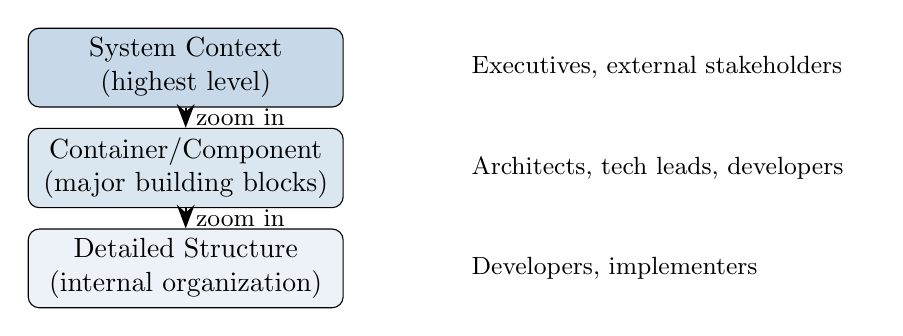
\begin{tikzpicture}[
    scale=0.85,
    level/.style={draw, rounded corners, minimum width=4cm, minimum height=1cm, align=center},
    arrow/.style={-{Stealth[length=3mm]}, thick}
]
    \node[level, fill=componentcolor!30] (l1) at (0,3) {System Context\\(highest level)};
    \node[level, fill=componentcolor!20] (l2) at (0,1.5) {Container/Component\\(major building blocks)};
    \node[level, fill=componentcolor!10] (l3) at (0,0) {Detailed Structure\\(internal organization)};
    
    \draw[arrow] (l1) -- node[right, font=\small] {zoom in} (l2);
    \draw[arrow] (l2) -- node[right, font=\small] {zoom in} (l3);
    
    \node[right=1.5cm of l1, text width=5cm, font=\small] {Executives, external stakeholders};
    \node[right=1.5cm of l2, text width=5cm, font=\small] {Architects, tech leads, developers};
    \node[right=1.5cm of l3, text width=5cm, font=\small] {Developers, implementers};
\end{tikzpicture}
\caption{Progressive Disclosure Hierarchy}
\end{figure}

\subsection{Consistency}

Consistency reduces cognitive load by allowing viewers to learn the notation once and apply it throughout.

\subsubsection{Internal Consistency}

Within a single diagram, maintain consistency in shape usage (same shapes for same element types), color coding (same colors for same categories), line styles (same styles for same relationship types), sizing (similar elements have similar sizes), labeling (same format and detail level for labels), and positioning (similar elements in similar positions).

\subsubsection{External Consistency}

Across diagrams within a documentation set, maintain consistency in notation conventions (use the same legend throughout), abstraction levels (similar detail at similar zoom levels), terminology (same names for same concepts), and visual style (consistent look and feel).

\subsection{Layout Strategies}

Effective layout makes diagrams easier to read and understand.

\subsubsection{Hierarchical Layout}

Use hierarchical layout for decomposition, containment, and dependency relationships. Parent elements at top, children below, with dependencies flowing downward.

\subsubsection{Layered Layout}

Use layered layout for architectural layers, protocol stacks, and abstract-to-concrete relationships. Higher abstraction at top, lower abstraction at bottom.

\subsubsection{Orthogonal Layout}

Use orthogonal (grid-based) layout for clarity in complex diagrams. Elements aligned to grid, connections using horizontal and vertical segments only.

\subsubsection{Circular/Radial Layout}

Use circular layout to show peer relationships or to highlight a central element with its connections.

\begin{bestpractice}
\textbf{Layout Guidelines:}
\begin{itemize}[nosep]
    \item Minimize line crossings---each crossing increases cognitive load
    \item Maintain consistent spacing between elements
    \item Align elements to an implicit grid
    \item Leave adequate white space---crowded diagrams are hard to read
    \item Place the most important elements prominently (center or top)
    \item Consider reading direction (left-to-right, top-to-bottom in Western cultures)
\end{itemize}
\end{bestpractice}

\subsection{Color Usage}

Color is a powerful visual channel but must be used carefully.

\begin{longtable}{@{}L{3cm} L{4cm} L{5.5cm}@{}}
\caption{Effective Color Usage} \\
\toprule
\textbf{Purpose} & \textbf{Approach} & \textbf{Guidelines} \\
\midrule
\endfirsthead
\toprule
\textbf{Purpose} & \textbf{Approach} & \textbf{Guidelines} \\
\midrule
\endhead
\bottomrule
\endlastfoot
Categorization & Distinct hues & Use 5--7 colors maximum; ensure adequate contrast \\
Layering & Value gradients & Darker for lower layers, lighter for higher \\
Status/State & Semantic colors & Red=error, yellow=warning, green=healthy \\
Emphasis & Saturation & Saturated for focus, desaturated for context \\
Grouping & Background fills & Light backgrounds for regions; consistent within groups \\
\end{longtable}

\begin{warning}
\textbf{Color Accessibility:}
\begin{itemize}[nosep]
    \item Approximately 8\% of men have color vision deficiency
    \item Never use color as the only distinguishing characteristic
    \item Combine color with shape, pattern, or label differences
    \item Test diagrams with color blindness simulators
    \item Ensure sufficient contrast for readability
\end{itemize}
\end{warning}

%==============================================================================
\section{Notation Standards and Conventions}
%==============================================================================

\subsection{Choosing a Notation}

The choice of notation affects how effectively the diagram communicates to its intended audience. Consider standardization (well-known notations reduce learning curve), expressiveness (the notation should represent needed concepts), tool support (modeling tools should support the notation), and audience familiarity (match notation to stakeholder expectations).

\subsection{UML for Architecture}

The Unified Modeling Language provides several diagram types useful for architectural documentation.

\subsubsection{UML Component Diagram}

\begin{figure}[H]
\centering
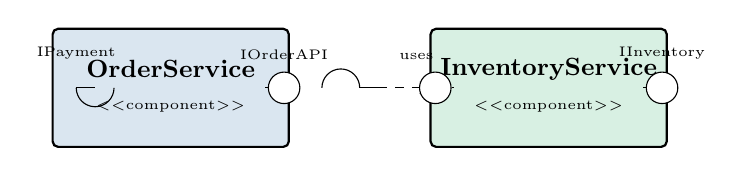
\begin{tikzpicture}[
    scale=0.8,
    component/.style={draw, thick, minimum width=3cm, minimum height=1.5cm, rounded corners=2pt},
    interface/.style={draw, fill=white, circle, minimum size=0.4cm},
    required/.style={draw, minimum size=0.4cm, semicircle, anchor=arc start},
    lollipop/.style={-},
    dependency/.style={-{Stealth[length=2mm]}, dashed}
]
    % Components
    \node[component, fill=componentcolor!20] (order) at (0,0) {};
    \node at (0,0.3) {\small\textbf{OrderService}};
    \node[font=\tiny] at (0,-0.3) {$<<$component$>>$};
    
    \node[component, fill=modulecolor!20] (inventory) at (6,0) {};
    \node at (6,0.3) {\small\textbf{InventoryService}};
    \node[font=\tiny] at (6,-0.3) {$<<$component$>>$};
    
    % Provided interfaces (lollipops)
    \node[interface] (orderapi) at (1.8,0) {};
    \draw[lollipop] (1.5,0) -- (orderapi);
    \node[font=\tiny, above] at (1.8,0.3) {IOrderAPI};
    
    \node[interface] (invapi) at (7.8,0) {};
    \draw[lollipop] (7.5,0) -- (invapi);
    \node[font=\tiny, above] at (7.8,0.3) {IInventory};
    
    % Required interface (socket)
    \draw (-1.5,0) arc (180:360:0.3);
    \draw (-1.5,0) -- (-1.2,0);
    \node[font=\tiny, above] at (-1.5,0.3) {IPayment};
    
    % Required interface on OrderService for Inventory
    \draw (3,0) arc (0:180:0.3);
    \draw (3,0) -- (3.3,0);
    
    % Dependency
    \draw[dependency] (3.3,0) -- (4.2,0);
    \node[interface] (invuse) at (4.2,0) {};
    \draw[lollipop] (invuse) -- (4.5,0);
    \node[font=\tiny, above] at (3.9,0.3) {uses};
\end{tikzpicture}
\caption{UML Component Diagram Notation}
\end{figure}

\subsubsection{UML Deployment Diagram}

\begin{longtable}{@{}C{2cm} L{3.5cm} L{7cm}@{}}
\caption{UML Deployment Diagram Elements} \\
\toprule
\textbf{Symbol} & \textbf{Name} & \textbf{Description} \\
\midrule
\endfirsthead
\toprule
\textbf{Symbol} & \textbf{Name} & \textbf{Description} \\
\midrule
\endhead
\bottomrule
\endlastfoot
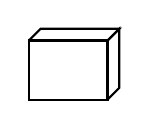
\begin{tikzpicture}[scale=0.5]
\draw[thick] (0,0) -- (2,0) -- (2,1.5) -- (0,1.5) -- cycle;
\draw[thick] (0,1.5) -- (0.3,1.8) -- (2.3,1.8) -- (2,1.5);
\draw[thick] (2,1.5) -- (2.3,1.8) -- (2.3,0.3) -- (2,0);
\end{tikzpicture}
& Node & Physical or virtual computing resource \\
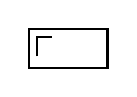
\begin{tikzpicture}[scale=0.5]
\draw[thick] (0,0) rectangle (2,1);
\draw[thick] (0.2,0.3) -- (0.2,0.8) -- (0.6,0.8);
\end{tikzpicture}
& Artifact & Deployable unit (JAR, WAR, executable) \\
\begin{tikzpicture}[scale=0.5]
\draw[thick, dashed] (0,0.5) -- (2,0.5);
\end{tikzpicture}
& Communication Path & Network connection between nodes \\
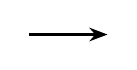
\begin{tikzpicture}[scale=0.5]
\draw[thick, -{Stealth}] (0,0.5) -- (2,0.5);
\end{tikzpicture}
& Deployment & Artifact deployed to node \\
\end{longtable}

\subsection{C4 Model Notation}

The C4 model provides a hierarchical approach with four levels: Context, Container, Component, and Code.

\begin{figure}[H]
\centering
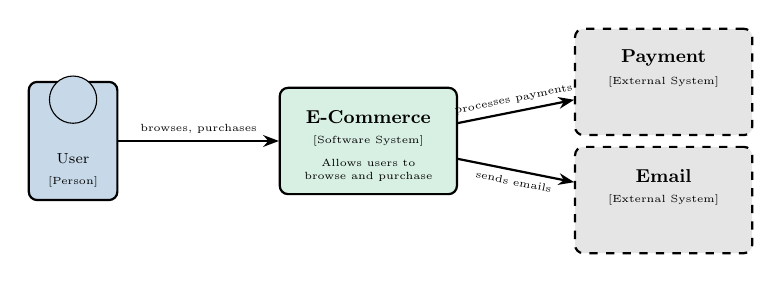
\begin{tikzpicture}[
    scale=0.75,
    transform shape,
    person/.style={draw, thick, fill=componentcolor!30, minimum width=1.5cm, minimum height=2cm, rounded corners=3pt},
    system/.style={draw, thick, fill=modulecolor!20, minimum width=3cm, minimum height=1.8cm, rounded corners=3pt},
    external/.style={draw, thick, fill=gray!20, minimum width=3cm, minimum height=1.8cm, rounded corners=3pt, dashed},
    container/.style={draw, thick, fill=servicecolor!20, minimum width=2.5cm, minimum height=1.5cm, rounded corners=3pt},
    relation/.style={-{Stealth[length=2mm]}, thick}
]
    % Person
    \node[person] (user) at (-5,0) {};
    \node[draw, fill=componentcolor!30, circle, minimum size=0.8cm] at (-5,0.7) {};
    \node[font=\scriptsize] at (-5,-0.3) {User};
    \node[font=\tiny] at (-5,-0.7) {[Person]};
    
    % Main system
    \node[system] (main) at (0,0) {};
    \node[font=\small\bfseries] at (0,0.4) {E-Commerce};
    \node[font=\tiny] at (0,0) {[Software System]};
    \node[font=\tiny, text width=2.5cm, align=center] at (0,-0.5) {Allows users to browse and purchase};
    
    % External systems
    \node[external] (payment) at (5,1) {};
    \node[font=\small\bfseries] at (5,1.4) {Payment};
    \node[font=\tiny] at (5,1) {[External System]};
    
    \node[external] (email) at (5,-1) {};
    \node[font=\small\bfseries] at (5,-0.6) {Email};
    \node[font=\tiny] at (5,-1) {[External System]};
    
    % Relations
    \draw[relation] (user) -- node[above, font=\tiny] {browses, purchases} (main);
    \draw[relation] (main) -- node[above, font=\tiny, sloped] {processes payments} (payment);
    \draw[relation] (main) -- node[below, font=\tiny, sloped] {sends emails} (email);
\end{tikzpicture}
\caption{C4 Context Diagram Notation}
\end{figure}

\subsubsection{C4 Notation Elements}

\begin{longtable}{@{}L{2.5cm} L{2.5cm} L{7.5cm}@{}}
\caption{C4 Model Element Types} \\
\toprule
\textbf{Element} & \textbf{Visual Style} & \textbf{Description} \\
\midrule
\endfirsthead
\toprule
\textbf{Element} & \textbf{Visual Style} & \textbf{Description} \\
\midrule
\endhead
\bottomrule
\endlastfoot
Person & Stick figure or labeled box & A human user of the system \\
Software System & Solid box with label & The system being described or an external system \\
Container & Solid box (different color) & An application or data store within the system \\
Component & Solid box (lighter) & A grouping of related functionality within a container \\
External System & Dashed box (gray) & A system outside your control \\
Relationship & Arrow with label & Describes the interaction between elements \\
\end{longtable}

\subsection{ArchiMate Notation}

ArchiMate provides enterprise architecture notation spanning business, application, and technology layers.

\begin{figure}[H]
\centering
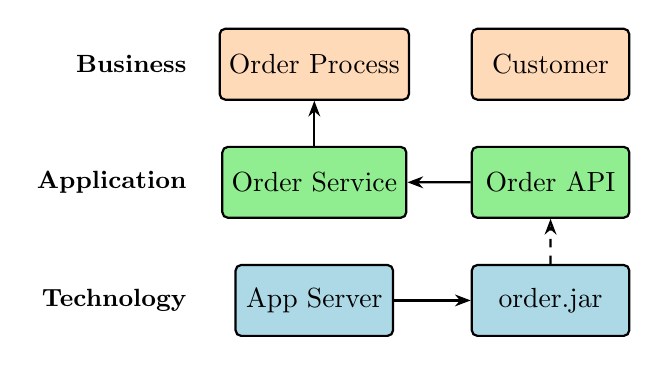
\begin{tikzpicture}[
    scale=0.75,
    business/.style={draw, thick, fill=layercolor3, minimum width=2cm, minimum height=0.9cm, rounded corners=2pt},
    application/.style={draw, thick, fill=layercolor2, minimum width=2cm, minimum height=0.9cm, rounded corners=2pt},
    technology/.style={draw, thick, fill=layercolor1, minimum width=2cm, minimum height=0.9cm, rounded corners=2pt},
    serving/.style={-{Stealth[length=2mm]}, thick},
    realization/.style={-{Stealth[length=2mm, open]}, thick, dashed}
]
    % Business layer
    \node[business] (process) at (0,4) {Order Process};
    \node[business] (role) at (4,4) {Customer};
    
    % Application layer
    \node[application] (service) at (0,2) {Order Service};
    \node[application] (component) at (4,2) {Order API};
    
    % Technology layer
    \node[technology] (node) at (0,0) {App Server};
    \node[technology] (artifact) at (4,0) {order.jar};
    
    % Relations
    \draw[serving] (service) -- (process);
    \draw[serving] (component) -- (service);
    \draw[realization] (artifact) -- (component);
    \draw[serving] (node) -- (artifact);
    
    % Layer labels
    \node[font=\small\bfseries, left] at (-2,4) {Business};
    \node[font=\small\bfseries, left] at (-2,2) {Application};
    \node[font=\small\bfseries, left] at (-2,0) {Technology};
\end{tikzpicture}
\caption{ArchiMate Cross-Layer Notation}
\end{figure}

\subsection{Custom Notation}

When standard notations are insufficient or inappropriate, custom notation may be used. However, custom notation requires careful documentation.

\begin{template}
\textbf{Custom Notation Documentation Requirements:}

For each custom element type:
\begin{itemize}[nosep]
    \item Visual representation (shape, color, border style)
    \item Semantic meaning (what it represents)
    \item Usage guidelines (when to use this element type)
    \item Examples (concrete instances)
\end{itemize}

For each custom relationship type:
\begin{itemize}[nosep]
    \item Visual representation (line style, arrowheads, decorations)
    \item Semantic meaning (what relationship it represents)
    \item Directionality (what source and target mean)
    \item Labels (what information goes on the line)
\end{itemize}
\end{template}

%==============================================================================
\section{Element Key and Legend Design}
%==============================================================================

\subsection{Purpose of the Legend}

Every primary presentation must include a legend (element key) that explains the notation used. The legend serves as a reference for interpreting the diagram, defines the visual vocabulary, ensures consistent interpretation across readers, and documents any non-standard notation.

\subsection{Legend Structure}

A comprehensive legend includes element types, relationship types, and any special annotations or conventions.

\begin{figure}[H]
\centering
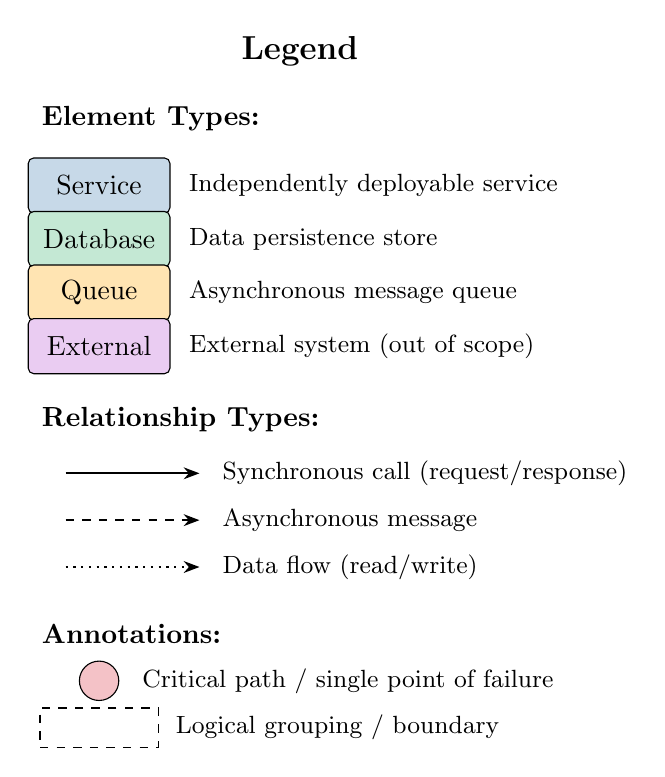
\begin{tikzpicture}[
    scale=0.85,
    elembox/.style={draw, minimum width=1.8cm, minimum height=0.7cm, rounded corners=2pt},
    relline/.style={minimum width=2cm}
]
    % Title
    \node[font=\large\bfseries] at (0,4.5) {Legend};
    
    % Element types section
    \node[font=\bfseries, anchor=west] at (-4,3.5) {Element Types:};
    
    \node[elembox, fill=componentcolor!30] at (-3,2.5) {Service};
    \node[anchor=west, font=\small] at (-1.8,2.5) {Independently deployable service};
    
    \node[elembox, fill=modulecolor!30] at (-3,1.7) {Database};
    \node[anchor=west, font=\small] at (-1.8,1.7) {Data persistence store};
    
    \node[elembox, fill=servicecolor!30] at (-3,0.9) {Queue};
    \node[anchor=west, font=\small] at (-1.8,0.9) {Asynchronous message queue};
    
    \node[elembox, fill=datacolor!30] at (-3,0.1) {External};
    \node[anchor=west, font=\small] at (-1.8,0.1) {External system (out of scope)};
    
    % Relationship types section
    \node[font=\bfseries, anchor=west] at (-4,-1) {Relationship Types:};
    
    \draw[-{Stealth[length=2mm]}, thick] (-3.5,-1.8) -- (-1.5,-1.8);
    \node[anchor=west, font=\small] at (-1.3,-1.8) {Synchronous call (request/response)};
    
    \draw[-{Stealth[length=2mm]}, thick, dashed] (-3.5,-2.5) -- (-1.5,-2.5);
    \node[anchor=west, font=\small] at (-1.3,-2.5) {Asynchronous message};
    
    \draw[-{Stealth[length=2mm]}, thick, dotted] (-3.5,-3.2) -- (-1.5,-3.2);
    \node[anchor=west, font=\small] at (-1.3,-3.2) {Data flow (read/write)};
    
    % Annotations section
    \node[font=\bfseries, anchor=west] at (-4,-4.2) {Annotations:};
    
    \node[draw, circle, fill=warningred!30, minimum size=0.5cm] at (-3,-4.9) {};
    \node[anchor=west, font=\small] at (-2.5,-4.9) {Critical path / single point of failure};
    
    \node[draw, dashed, minimum width=1.5cm, minimum height=0.5cm] at (-3,-5.6) {};
    \node[anchor=west, font=\small] at (-2,-5.6) {Logical grouping / boundary};
\end{tikzpicture}
\caption{Comprehensive Legend Example}
\end{figure}

\subsection{Element Type Documentation}

For each element type in the legend, document the visual representation, semantic meaning, typical properties, and examples from this diagram.

\setlength{\extrarowheight}{4pt}
\begin{longtable}{@{}L{2cm} C{2.5cm} L{4cm} L{4cm}@{}}
\caption{Element Type Documentation Template} \\
\toprule
\textbf{Type Name} & \textbf{Visual} & \textbf{Meaning} & \textbf{Examples} \\
\midrule
\endfirsthead
\toprule
\textbf{Type Name} & \textbf{Visual} & \textbf{Meaning} & \textbf{Examples} \\
\midrule
\endhead
\bottomrule
\endlastfoot
Service & \tikz{\node[draw, fill=componentcolor!30, minimum width=1.2cm, minimum height=0.5cm, rounded corners=2pt, font=\tiny] {Service};} & Independently deployable unit providing business capability & Order Service, Payment Service \\
Database & \tikz{\node[draw, fill=datacolor!30, cylinder, shape border rotate=90, aspect=0.4, minimum width=0.8cm, minimum height=0.5cm, font=\tiny] {};} & Persistent data storage with query capability & OrderDB, UserDB \\
Queue & \tikz{\node[draw, fill=servicecolor!30, minimum width=1.2cm, minimum height=0.4cm, rounded corners=2pt, font=\tiny] {Queue};} & Asynchronous message buffer & Event Bus, Task Queue \\
External & \tikz{\node[draw, dashed, fill=gray!20, minimum width=1.2cm, minimum height=0.5cm, rounded corners=2pt, font=\tiny] {External};} & System outside our control & Payment Gateway, Email Provider \\
\end{longtable}

\subsection{Relationship Type Documentation}

\begin{longtable}{@{}L{2.2cm} C{2.5cm} L{4cm} L{4cm}@{}}
\caption{Relationship Type Documentation Template} \\
\toprule
\textbf{Type} & \textbf{Visual} & \textbf{Meaning} & \textbf{Examples} \\
\midrule
\endfirsthead
\toprule
\textbf{Type} & \textbf{Visual} & \textbf{Meaning} & \textbf{Examples} \\
\midrule
\endhead
\bottomrule
\endlastfoot
Sync Call & \tikz{\draw[-{Stealth[length=2mm]}, thick] (0,0) -- (1.5,0);} & Synchronous request-response invocation & API calls, RPC \\
Async Message & \tikz{\draw[-{Stealth[length=2mm]}, thick, dashed] (0,0) -- (1.5,0);} & Fire-and-forget or pub/sub message & Events, commands \\
Data Flow & \tikz{\draw[-{Stealth[length=2mm]}, thick, dotted] (0,0) -- (1.5,0);} & Data transfer (read or write) & DB queries, file writes \\
Dependency & \tikz{\draw[-{Stealth[length=2mm, open]}, thick] (0,0) -- (1.5,0);} & Compile-time or structural dependency & Uses, imports \\
Contains & \tikz{\draw[-{Diamond[length=3mm]}, thick] (1.5,0) -- (0,0);} & Composition / containment & Module contains class \\
\end{longtable}

%==============================================================================
\section{Narrative Description Techniques}
%==============================================================================

\subsection{The Role of Narrative}

The narrative description is a textual walkthrough that guides readers through the primary presentation. It complements the visual diagram by explaining intent, significance, and context that cannot be conveyed visually.

\begin{keypoint}
The narrative should answer questions the diagram raises but cannot answer: Why is the system structured this way? What are the significant design decisions? How does this structure support quality attributes?
\end{keypoint}

\subsection{Narrative Structure}

An effective narrative follows a logical structure that builds understanding progressively.

\begin{enumerate}
    \item \textbf{Overview:} Start with a one-paragraph summary of what the diagram shows
    \item \textbf{Major Elements:} Describe the primary elements and their responsibilities
    \item \textbf{Key Relationships:} Explain the most important interactions and dependencies
    \item \textbf{Data and Control Flow:} Describe how data and control move through the structure
    \item \textbf{Quality Attribute Support:} Explain how the structure supports key quality attributes
    \item \textbf{Notable Decisions:} Highlight significant design decisions and their rationale
\end{enumerate}

\subsection{Writing Effective Narratives}

\begin{bestpractice}
\textbf{Narrative Writing Guidelines:}

\textbf{Be purposeful:} Every sentence should add value. Avoid restating what is obvious from the diagram.

\textbf{Use consistent terminology:} Use element names exactly as they appear in the diagram.

\textbf{Explain significance:} Don't just describe what is shown; explain why it matters.

\textbf{Connect to concerns:} Relate structural choices to stakeholder concerns and quality attributes.

\textbf{Be concrete:} Use specific examples of scenarios and interactions.

\textbf{Maintain appropriate detail:} Match detail level to audience; don't overwhelm with implementation specifics.
\end{bestpractice}

\subsection{Narrative Example}

\begin{example}
\textbf{Narrative for Service-Oriented Architecture Diagram}

\vspace{0.2cm}
\textbf{Overview:} This diagram presents the runtime structure of the e-commerce platform as a collection of independently deployable services communicating through synchronous APIs and asynchronous events.

\vspace{0.2cm}
\textbf{Major Elements:} The system consists of four primary services. The \textit{API Gateway} serves as the single entry point for all client requests, handling authentication, rate limiting, and request routing. The \textit{Order Service} manages the complete order lifecycle from creation through fulfillment. The \textit{Inventory Service} maintains real-time inventory levels and handles stock reservations. The \textit{Payment Service} processes payments through integration with external payment providers.

\vspace{0.2cm}
\textbf{Key Relationships:} The API Gateway routes all external requests to appropriate backend services, providing a unified interface while hiding internal complexity. The Order Service orchestrates order creation by coordinating with Inventory (to reserve stock) and Payment (to process charges) services. All services publish domain events to the Event Bus, enabling loose coupling and eventual consistency.

\vspace{0.2cm}
\textbf{Quality Attribute Support:} This structure supports several key quality attributes. \textit{Availability} is enhanced through service independence---failure of the Payment Service does not affect product browsing. \textit{Scalability} is achieved by allowing individual services to scale independently based on their specific load. \textit{Modifiability} benefits from clear service boundaries---changes to payment processing are isolated to one service.

\vspace{0.2cm}
\textbf{Notable Decisions:} The choice of asynchronous events for inter-service communication (rather than synchronous calls for everything) was driven by resilience requirements. Services can continue operating during temporary unavailability of other services, with events queued for later processing.
\end{example}

%==============================================================================
\section{Behavioral Overview Integration}
%==============================================================================

\subsection{Static vs. Dynamic Views}

The primary presentation typically shows static structure---elements and their relationships at rest. However, architecture is also about behavior---how elements interact over time. The behavioral overview bridges this gap.

\subsection{Behavioral Summary Approaches}

\subsubsection{Scenario Walkthroughs}

Describe key scenarios as sequences of interactions through the structure.

\begin{example}
\textbf{Scenario: Customer Places Order}

\begin{enumerate}[nosep]
    \item Customer submits order through Web UI to API Gateway
    \item API Gateway authenticates request and routes to Order Service
    \item Order Service validates order and requests inventory reservation from Inventory Service
    \item Inventory Service reserves stock and returns confirmation
    \item Order Service requests payment processing from Payment Service
    \item Payment Service processes payment through external gateway
    \item Order Service publishes OrderCreated event to Event Bus
    \item Notification Service (subscribed to events) sends confirmation email
\end{enumerate}
\end{example}

\subsubsection{Interaction Diagrams}

Reference supporting sequence or collaboration diagrams that detail important interactions.

\begin{figure}[H]
\centering
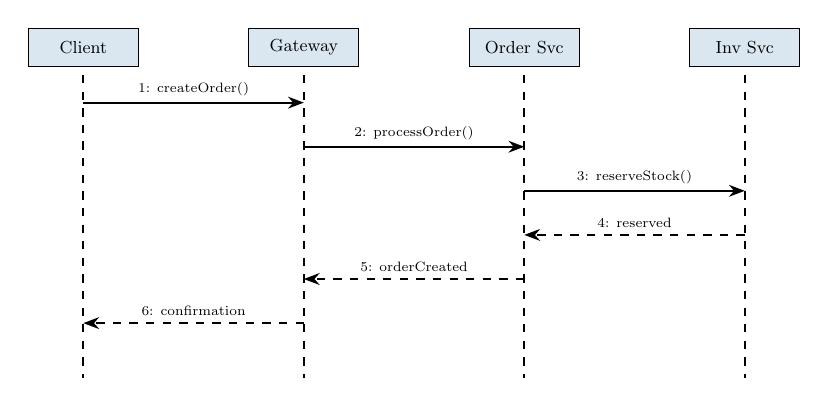
\begin{tikzpicture}[
    scale=0.7,
    transform shape,
    participant/.style={draw, fill=componentcolor!20, minimum width=2cm, minimum height=0.7cm, font=\small},
    lifeline/.style={dashed, thick},
    message/.style={-{Stealth[length=2mm]}, thick},
    return/.style={-{Stealth[length=2mm]}, thick, dashed}
]
    % Participants
    \node[participant] (client) at (0,0) {Client};
    \node[participant] (gateway) at (4,0) {Gateway};
    \node[participant] (order) at (8,0) {Order Svc};
    \node[participant] (inv) at (12,0) {Inv Svc};
    
    % Lifelines
    \draw[lifeline] (0,-0.5) -- (0,-6);
    \draw[lifeline] (4,-0.5) -- (4,-6);
    \draw[lifeline] (8,-0.5) -- (8,-6);
    \draw[lifeline] (12,-0.5) -- (12,-6);
    
    % Messages
    \draw[message] (0,-1) -- node[above, font=\scriptsize] {1: createOrder()} (4,-1);
    \draw[message] (4,-1.8) -- node[above, font=\scriptsize] {2: processOrder()} (8,-1.8);
    \draw[message] (8,-2.6) -- node[above, font=\scriptsize] {3: reserveStock()} (12,-2.6);
    \draw[return] (12,-3.4) -- node[above, font=\scriptsize] {4: reserved} (8,-3.4);
    \draw[return] (8,-4.2) -- node[above, font=\scriptsize] {5: orderCreated} (4,-4.2);
    \draw[return] (4,-5) -- node[above, font=\scriptsize] {6: confirmation} (0,-5);
\end{tikzpicture}
\caption{Order Creation Sequence (Simplified)}
\end{figure}

\subsubsection{State and Lifecycle}

For elements with significant state, summarize their lifecycle.

\begin{longtable}{@{}L{2.5cm} L{3.5cm} L{6.5cm}@{}}
\caption{Element Lifecycle Summary} \\
\toprule
\textbf{Element} & \textbf{Key States} & \textbf{Lifecycle Notes} \\
\midrule
\endfirsthead
\toprule
\textbf{Element} & \textbf{Key States} & \textbf{Lifecycle Notes} \\
\midrule
\endhead
\bottomrule
\endlastfoot
Order Service & Starting, Ready, Degraded, Stopping & Starts with database connection; enters Degraded if DB unavailable \\
Order Entity & Pending, Confirmed, Shipped, Delivered, Cancelled & Transitions driven by events; terminal states are Delivered, Cancelled \\
Inventory Reservation & Pending, Committed, Released & 15-minute timeout on Pending; auto-release if not committed \\
\end{longtable}

\subsection{Behavioral References}

Link to detailed behavioral models maintained separately.

\begin{longtable}{@{}L{3.5cm} L{3cm} L{6cm}@{}}
\caption{Behavioral Model References} \\
\toprule
\textbf{Scenario/Behavior} & \textbf{Model Type} & \textbf{Reference} \\
\midrule
\endfirsthead
\toprule
\textbf{Scenario/Behavior} & \textbf{Model Type} & \textbf{Reference} \\
\midrule
\endhead
\bottomrule
\endlastfoot
Order Creation Flow & Sequence Diagram & [DOC:behavior/seq-order-create.md] \\
Order Cancellation & Sequence Diagram & [DOC:behavior/seq-order-cancel.md] \\
Payment Processing & Activity Diagram & [DOC:behavior/act-payment.md] \\
Order State Machine & State Diagram & [DOC:behavior/state-order.md] \\
Inventory Saga & Saga Diagram & [DOC:behavior/saga-inventory.md] \\
\end{longtable}

%==============================================================================
\section{Constraints and Design Rules}
%==============================================================================

\subsection{Purpose of Documented Constraints}

Constraints and design rules are architectural decisions that restrict how elements may be used, connected, or changed. Documenting these rules in the primary presentation ensures that implementers understand and follow the intended architecture.

\subsection{Types of Constraints}

\subsubsection{Structural Constraints}

Structural constraints govern how elements may be organized and related.

\begin{longtable}{@{}L{3cm} L{5cm} L{4.5cm}@{}}
\caption{Structural Constraints} \\
\toprule
\textbf{Constraint Type} & \textbf{Description} & \textbf{Example} \\
\midrule
\endfirsthead
\toprule
\textbf{Constraint Type} & \textbf{Description} & \textbf{Example} \\
\midrule
\endhead
\bottomrule
\endlastfoot
Layering Rules & Allowed dependencies between layers & UI layer may only call Application layer \\
Containment Rules & What may contain what & Services contain components; components contain classes \\
Cardinality & Required number of elements & Each service must have exactly one database \\
Exclusion & Elements that may not coexist & Synchronous and async variants of same interface \\
Required Elements & Elements that must exist & Every service must have health check endpoint \\
\end{longtable}

\subsubsection{Communication Constraints}

Communication constraints govern how elements may interact.

\begin{longtable}{@{}L{3cm} L{5cm} L{4.5cm}@{}}
\caption{Communication Constraints} \\
\toprule
\textbf{Constraint Type} & \textbf{Description} & \textbf{Example} \\
\midrule
\endfirsthead
\toprule
\textbf{Constraint Type} & \textbf{Description} & \textbf{Example} \\
\midrule
\endhead
\bottomrule
\endlastfoot
Protocol Requirements & Required communication protocols & All service-to-service calls use gRPC \\
Direction Rules & Allowed call directions & Services may not call the API Gateway \\
Intermediary Requirements & Required intermediate elements & All external calls must go through Gateway \\
Async Requirements & When async is required & Cross-domain communication must be async \\
\end{longtable}

\subsubsection{Technology Constraints}

Technology constraints mandate or prohibit specific technologies.

\begin{longtable}{@{}L{3cm} L{5cm} L{4.5cm}@{}}
\caption{Technology Constraints} \\
\toprule
\textbf{Constraint Type} & \textbf{Description} & \textbf{Example} \\
\midrule
\endfirsthead
\toprule
\textbf{Constraint Type} & \textbf{Description} & \textbf{Example} \\
\midrule
\endhead
\bottomrule
\endlastfoot
Language/Framework & Mandated or prohibited technologies & Services must use Java or Go \\
Data Stores & Allowed database technologies & Relational data uses PostgreSQL only \\
Infrastructure & Required platforms & All services deploy to Kubernetes \\
Libraries & Mandated libraries for cross-cutting concerns & All services use OpenTelemetry for tracing \\
\end{longtable}

\subsection{Constraint Documentation Format}

\begin{template}
\textbf{Constraint Specification Template}

\vspace{0.2cm}
\textbf{Constraint ID:} Unique identifier

\textbf{Name:} Short descriptive name

\textbf{Category:} Structural / Communication / Technology / Quality

\textbf{Statement:} Precise statement of the constraint

\textbf{Rationale:} Why this constraint exists

\textbf{Enforcement:} How the constraint is enforced (review, tooling, tests)

\textbf{Exceptions:} Any allowed exceptions and approval process

\textbf{Related Decisions:} Link to architectural decision record
\end{template}

\subsection{Example Constraints}

\begin{tcolorbox}[colback=lightgray, colframe=sectionblue, title=\textbf{Constraint: LAYER-001 -- Layer Dependency Direction}]

\textbf{Statement:} Dependencies between layers must flow downward only. A higher layer may depend on a lower layer, but a lower layer may not depend on a higher layer.

\vspace{0.2cm}
\textbf{Rationale:} Enforcing unidirectional dependencies ensures that lower layers remain stable and reusable. Changes to the UI layer should not require changes to business logic or data access layers.

\vspace{0.2cm}
\textbf{Enforcement:} 
\begin{itemize}[nosep]
    \item Static analysis tools (ArchUnit, NDepend) run in CI pipeline
    \item Architecture review checklist includes dependency verification
    \item Violations fail the build
\end{itemize}

\vspace{0.2cm}
\textbf{Exceptions:} Dependency inversion through interfaces is allowed (lower layer defines interface, higher layer implements). Must be documented in element catalog.
\end{tcolorbox}

\begin{tcolorbox}[colback=lightgray, colframe=sectionblue, title=\textbf{Constraint: COMM-003 -- Cross-Domain Async Requirement}]

\textbf{Statement:} Communication between services in different business domains must use asynchronous messaging via the Event Bus. Synchronous calls are prohibited.

\vspace{0.2cm}
\textbf{Rationale:} Asynchronous communication between domains reduces coupling, improves resilience (services can operate during partner unavailability), and supports independent scaling and deployment.

\vspace{0.2cm}
\textbf{Enforcement:}
\begin{itemize}[nosep]
    \item Service mesh policies reject cross-domain synchronous calls
    \item Architecture review for new integrations
    \item Domain boundary documentation maintained
\end{itemize}

\vspace{0.2cm}
\textbf{Exceptions:} Time-critical operations (payment confirmation) may use synchronous calls with architecture board approval. Must implement circuit breaker pattern.
\end{tcolorbox}

%==============================================================================
\section{Quality Attribute Visualization}
%==============================================================================

\subsection{Making Quality Attributes Visible}

While structure is the primary focus of architectural diagrams, quality attributes often drive structural decisions. Making quality considerations visible helps stakeholders understand why the architecture is designed as it is.

\subsection{Visual Annotation Techniques}

\subsubsection{Color Coding for Criticality}

\begin{figure}[H]
\centering
\begin{tikzpicture}[
    scale=0.75,
    service/.style={draw, thick, minimum width=2.2cm, minimum height=1cm, rounded corners=3pt}
]
    \node[service, fill=warningred!40] (gateway) at (0,2) {API Gateway};
    \node[service, fill=warningred!40] (order) at (-3,0) {Order Svc};
    \node[service, fill=highyellow!40] (inv) at (0,0) {Inventory};
    \node[service, fill=successgreen!20] (notify) at (3,0) {Notify Svc};
    
    % Legend
    \node[font=\small\bfseries] at (7,2) {Criticality:};
    \node[service, fill=warningred!40, minimum width=1.5cm, minimum height=0.5cm] at (6,1.2) {};
    \node[font=\scriptsize, right] at (7,1.2) {Critical};
    \node[service, fill=highyellow!40, minimum width=1.5cm, minimum height=0.5cm] at (6,0.5) {};
    \node[font=\scriptsize, right] at (7,0.5) {High};
    \node[service, fill=successgreen!20, minimum width=1.5cm, minimum height=0.5cm] at (6,-0.2) {};
    \node[font=\scriptsize, right] at (7,-0.2) {Low};
\end{tikzpicture}
\caption{Criticality Visualization}
\end{figure}

\subsubsection{Annotations for Performance}

Add performance annotations directly to elements or relationships.

\begin{figure}[H]
\centering
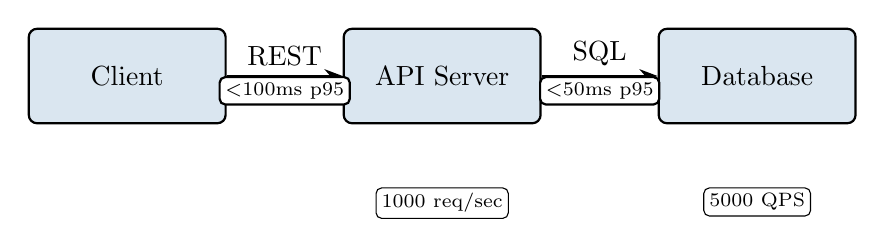
\begin{tikzpicture}[
    scale=0.8,
    service/.style={draw, thick, fill=componentcolor!20, minimum width=2.5cm, minimum height=1.2cm, rounded corners=3pt},
    perf/.style={font=\scriptsize, fill=white, draw, rounded corners=2pt, inner sep=2pt}
]
    \node[service] (client) at (0,0) {Client};
    \node[service] (api) at (5,0) {API Server};
    \node[service] (db) at (10,0) {Database};
    
    \draw[-{Stealth}, thick] (client) -- node[above] {REST} node[below, perf] {$<$100ms p95} (api);
    \draw[-{Stealth}, thick] (api) -- node[above] {SQL} node[below, perf] {$<$50ms p95} (db);
    
    \node[perf, below=0.8cm of api] {1000 req/sec};
    \node[perf, below=0.8cm of db] {5000 QPS};
\end{tikzpicture}
\caption{Performance Annotations}
\end{figure}

\subsubsection{Security Zone Boundaries}

\begin{figure}[H]
\centering
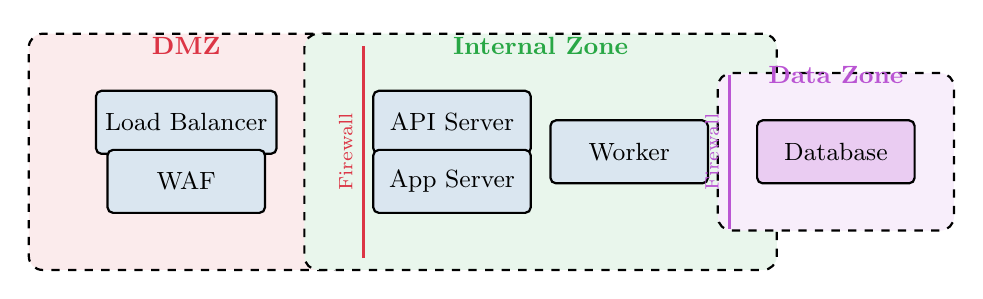
\begin{tikzpicture}[
    scale=0.75,
    zone/.style={draw, thick, dashed, rounded corners=5pt},
    service/.style={draw, thick, fill=componentcolor!20, minimum width=2cm, minimum height=0.8cm, rounded corners=2pt, font=\small}
]
    % Zones
    \node[zone, fill=warningred!10, minimum width=4cm, minimum height=3cm] (dmz) at (-3,0) {};
    \node[font=\small\bfseries, warningred] at (-3,1.8) {DMZ};
    
    \node[zone, fill=successgreen!10, minimum width=6cm, minimum height=3cm] (internal) at (3,0) {};
    \node[font=\small\bfseries, successgreen] at (3,1.8) {Internal Zone};
    
    \node[zone, fill=datacolor!10, minimum width=3cm, minimum height=2cm] (data) at (8,0) {};
    \node[font=\small\bfseries, datacolor] at (8,1.3) {Data Zone};
    
    % Services
    \node[service] (lb) at (-3,0.5) {Load Balancer};
    \node[service] (waf) at (-3,-0.5) {WAF};
    
    \node[service] (api) at (1.5,0.5) {API Server};
    \node[service] (app) at (1.5,-0.5) {App Server};
    \node[service] (worker) at (4.5,0) {Worker};
    
    \node[service, fill=datacolor!30] (db) at (8,0) {Database};
    
    % Firewall indicators
    \draw[very thick, warningred] (0,-1.8) -- (0,1.8);
    \node[font=\scriptsize, warningred, rotate=90] at (-0.3,0) {Firewall};
    
    \draw[very thick, datacolor] (6.2,-1.3) -- (6.2,1.3);
    \node[font=\scriptsize, datacolor, rotate=90] at (5.9,0) {Firewall};
\end{tikzpicture}
\caption{Security Zone Visualization}
\end{figure}

\subsubsection{Redundancy and Failover}

\begin{figure}[H]
\centering
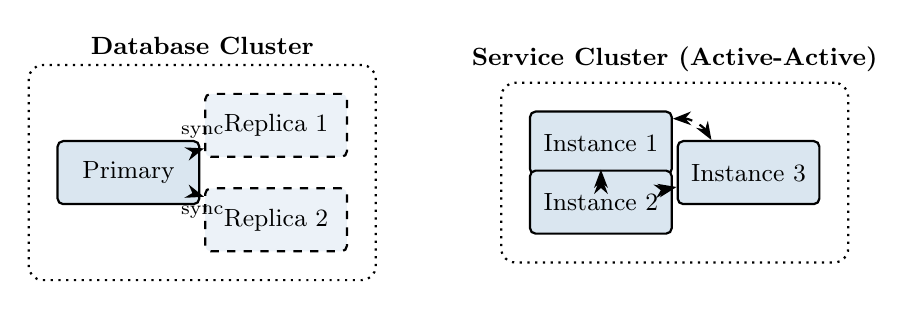
\begin{tikzpicture}[
    scale=0.75,
    instance/.style={draw, thick, fill=componentcolor!20, minimum width=1.8cm, minimum height=0.8cm, rounded corners=2pt, font=\small},
    replica/.style={draw, thick, fill=componentcolor!10, minimum width=1.8cm, minimum height=0.8cm, rounded corners=2pt, font=\small, dashed},
    cluster/.style={draw, thick, dotted, rounded corners=5pt}
]
    % Primary-Replica pattern
    \node[instance] (primary) at (0,0) {Primary};
    \node[replica] (replica1) at (2.5,0.8) {Replica 1};
    \node[replica] (replica2) at (2.5,-0.8) {Replica 2};
    
    \draw[-{Stealth}, thick] (primary) -- node[above, font=\scriptsize] {sync} (replica1);
    \draw[-{Stealth}, thick] (primary) -- node[below, font=\scriptsize] {sync} (replica2);
    
    % Cluster
    \node[cluster, fit=(primary)(replica1)(replica2), inner sep=10pt, label={[font=\small\bfseries]above:Database Cluster}] {};
    
    % Active-Active pattern
    \node[instance] (active1) at (8,0.5) {Instance 1};
    \node[instance] (active2) at (8,-0.5) {Instance 2};
    \node[instance] (active3) at (10.5,0) {Instance 3};
    
    \draw[{Stealth}-{Stealth}, thick, dashed] (active1) -- (active2);
    \draw[{Stealth}-{Stealth}, thick, dashed] (active2) -- (active3);
    \draw[{Stealth}-{Stealth}, thick, dashed] (active1) to[bend left] (active3);
    
    \node[cluster, fit=(active1)(active2)(active3), inner sep=10pt, label={[font=\small\bfseries]above:Service Cluster (Active-Active)}] {};
\end{tikzpicture}
\caption{Redundancy and Failover Patterns}
\end{figure}

\subsection{Quality Attribute Summary Table}

Include a summary table linking structural elements to quality attributes.

\begin{longtable}{@{}L{2.5cm} L{2cm} L{2cm} L{2cm} L{3.5cm}@{}}
\caption{Quality Attribute Summary by Element} \\
\toprule
\textbf{Element} & \textbf{Avail.} & \textbf{Perf.} & \textbf{Security} & \textbf{Notes} \\
\midrule
\endfirsthead
\toprule
\textbf{Element} & \textbf{Avail.} & \textbf{Perf.} & \textbf{Security} & \textbf{Notes} \\
\midrule
\endhead
\bottomrule
\endlastfoot
API Gateway & 99.99\% & $<$50ms & TLS, Auth & Redundant; rate limiting \\
Order Service & 99.95\% & $<$200ms & Internal & 3 replicas; circuit breaker \\
Database & 99.99\% & $<$10ms & Encrypted & Primary + 2 replicas \\
Event Bus & 99.9\% & best effort & Internal & 3-node Kafka cluster \\
\end{longtable}

%==============================================================================
\section{Known Issues and Future Work}
%==============================================================================

\subsection{Purpose of Issue Documentation}

Documenting known issues and incomplete areas is essential for honest communication with stakeholders. It sets appropriate expectations, identifies areas needing attention, and provides context for future work.

\subsection{Issue Categories}

\subsubsection{Accuracy Issues}

The diagram does not fully represent the current or intended state.

\begin{longtable}{@{}L{1cm} L{3.5cm} L{4cm} L{4cm}@{}}
\caption{Accuracy Issues} \\
\toprule
\textbf{ID} & \textbf{Issue} & \textbf{Impact} & \textbf{Resolution Plan} \\
\midrule
\endfirsthead
\toprule
\textbf{ID} & \textbf{Issue} & \textbf{Impact} & \textbf{Resolution Plan} \\
\midrule
\endhead
\bottomrule
\endlastfoot
A1 & Legacy Order Service not shown & Incomplete picture of dependencies & Add to diagram Q2 \\
A2 & Cache layer omitted for simplicity & May confuse performance analysis & Add cache to v2.0 \\
\end{longtable}

\subsubsection{Completeness Issues}

Areas that are not yet fully documented or designed.

\begin{longtable}{@{}L{1cm} L{3.5cm} L{4cm} L{4cm}@{}}
\caption{Completeness Issues} \\
\toprule
\textbf{ID} & \textbf{Issue} & \textbf{Impact} & \textbf{Resolution Plan} \\
\midrule
\endfirsthead
\toprule
\textbf{ID} & \textbf{Issue} & \textbf{Impact} & \textbf{Resolution Plan} \\
\midrule
\endhead
\bottomrule
\endlastfoot
C1 & Mobile backend not designed & Mobile integration unclear & Design sprint scheduled \\
C2 & Disaster recovery not shown & Operational gaps & DR architecture in progress \\
\end{longtable}

\subsubsection{Pending Decisions}

Architectural decisions that affect the diagram but are not yet made.

\begin{longtable}{@{}L{1cm} L{3.5cm} L{4cm} L{4cm}@{}}
\caption{Pending Decisions} \\
\toprule
\textbf{ID} & \textbf{Decision Needed} & \textbf{Diagram Impact} & \textbf{Target Date} \\
\midrule
\endfirsthead
\toprule
\textbf{ID} & \textbf{Decision Needed} & \textbf{Diagram Impact} & \textbf{Target Date} \\
\midrule
\endhead
\bottomrule
\endlastfoot
D1 & Event bus technology selection & May change connector notation & March 15 \\
D2 & Multi-region strategy & Major structural changes & April 1 \\
\end{longtable}

%==============================================================================
\section{Diagram Maintenance and Governance}
%==============================================================================

\subsection{Keeping Diagrams Current}

Diagrams that don't match reality are worse than no diagrams---they actively mislead. Establishing governance processes ensures diagrams remain accurate and useful.

\subsection{Update Triggers}

Diagrams should be updated when new elements are added to the system, elements are removed or deprecated, relationships between elements change, quality attribute requirements change significantly, technology choices change, and organizational boundaries change (for work assignment views).

\subsection{Review Process}

\begin{enumerate}
    \item \textbf{Scheduled Reviews:} Quarterly reviews of all primary presentations
    \item \textbf{Change-Triggered Reviews:} Review after significant system changes
    \item \textbf{Stakeholder Feedback:} Process for stakeholders to report inaccuracies
    \item \textbf{Implementation Comparison:} Periodic comparison with actual implementation
\end{enumerate}

\subsection{Version Control}

\begin{longtable}{@{}L{1.5cm} L{2cm} L{2.5cm} L{6.5cm}@{}}
\caption{Diagram Version History} \\
\toprule
\textbf{Version} & \textbf{Date} & \textbf{Author} & \textbf{Changes} \\
\midrule
\endfirsthead
\toprule
\textbf{Version} & \textbf{Date} & \textbf{Author} & \textbf{Changes} \\
\midrule
\endhead
\bottomrule
\endlastfoot
1.0 & 2024-01-15 & J. Smith & Initial diagram \\
1.1 & 2024-02-20 & A. Jones & Added Event Bus; updated service names \\
1.2 & 2024-03-15 & J. Smith & Added caching layer; updated legend \\
2.0 & 2024-06-01 & Architecture Team & Major revision for microservices migration \\
\end{longtable}

\subsection{Tooling Recommendations}

\begin{longtable}{@{}L{3cm} L{3.5cm} L{6cm}@{}}
\caption{Diagramming Tool Comparison} \\
\toprule
\textbf{Tool} & \textbf{Strengths} & \textbf{Best For} \\
\midrule
\endfirsthead
\toprule
\textbf{Tool} & \textbf{Strengths} & \textbf{Best For} \\
\midrule
\endhead
\bottomrule
\endlastfoot
Structurizr & C4 model; diagram-as-code; versioning & Teams adopting C4; code-first approach \\
Lucidchart & Collaborative; polished output; templates & Distributed teams; executive presentations \\
draw.io & Free; version control friendly; flexible & Budget-conscious; Git integration \\
PlantUML & Text-based; automated generation; CI-friendly & Developer documentation; automation \\
Miro & Collaborative whiteboarding; flexible & Workshops; brainstorming; informal \\
Enterprise Architect & Full UML; model repository; traceability & Large enterprises; formal modeling \\
\end{longtable}

%==============================================================================
\section{Appendix A: Notation Quick Reference}
%==============================================================================

\begin{figure}[H]
\centering
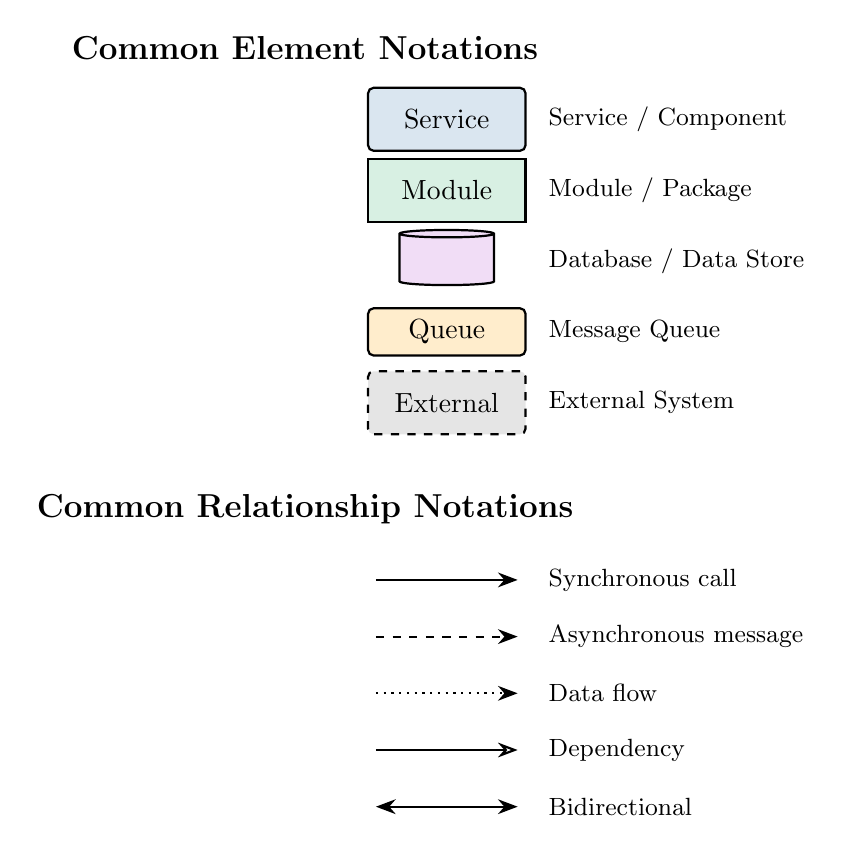
\begin{tikzpicture}[scale=0.9]
    % Element types
    \node[font=\large\bfseries] at (-2,5) {Common Element Notations};
    
    \node[draw, thick, fill=componentcolor!20, minimum width=2cm, minimum height=0.8cm, rounded corners=2pt] at (0,4) {Service};
    \node[right, font=\small] at (1.3,4) {Service / Component};
    
    \node[draw, thick, fill=modulecolor!20, minimum width=2cm, minimum height=0.8cm] at (0,3) {Module};
    \node[right, font=\small] at (1.3,3) {Module / Package};
    
    \node[draw, thick, fill=datacolor!20, cylinder, shape border rotate=90, aspect=0.4, minimum width=1.2cm, minimum height=0.7cm] at (0,2) {};
    \node[right, font=\small] at (1.3,2) {Database / Data Store};
    
    \node[draw, thick, fill=servicecolor!20, minimum width=2cm, minimum height=0.6cm, rounded corners=2pt] at (0,1) {Queue};
    \node[right, font=\small] at (1.3,1) {Message Queue};
    
    \node[draw, thick, dashed, fill=gray!20, minimum width=2cm, minimum height=0.8cm, rounded corners=2pt] at (0,0) {External};
    \node[right, font=\small] at (1.3,0) {External System};
    
    % Relationship types
    \node[font=\large\bfseries] at (-2,-1.5) {Common Relationship Notations};
    
    \draw[-{Stealth[length=2.5mm]}, thick] (-1,-2.5) -- (1,-2.5);
    \node[right, font=\small] at (1.3,-2.5) {Synchronous call};
    
    \draw[-{Stealth[length=2.5mm]}, thick, dashed] (-1,-3.3) -- (1,-3.3);
    \node[right, font=\small] at (1.3,-3.3) {Asynchronous message};
    
    \draw[-{Stealth[length=2.5mm]}, thick, dotted] (-1,-4.1) -- (1,-4.1);
    \node[right, font=\small] at (1.3,-4.1) {Data flow};
    
    \draw[-{Stealth[length=2.5mm, open]}, thick] (-1,-4.9) -- (1,-4.9);
    \node[right, font=\small] at (1.3,-4.9) {Dependency};
    
    \draw[{Stealth[length=2.5mm]}-{Stealth[length=2.5mm]}, thick] (-1,-5.7) -- (1,-5.7);
    \node[right, font=\small] at (1.3,-5.7) {Bidirectional};
\end{tikzpicture}
\caption{Notation Quick Reference}
\end{figure}

%==============================================================================
\section{Appendix B: Primary Presentation Checklist}
%==============================================================================

\subsection{Completeness Checklist}

\begin{itemize}[leftmargin=2cm]
    \item[$\square$] All significant elements from the view are shown
    \item[$\square$] All significant relationships are shown
    \item[$\square$] Element names match catalog entries
    \item[$\square$] Legend/key explains all notation used
    \item[$\square$] Diagram has descriptive title
    \item[$\square$] Version and date are indicated
    \item[$\square$] Narrative description is provided
    \item[$\square$] Constraints and rules are documented
    \item[$\square$] Known issues are documented
\end{itemize}

\subsection{Quality Checklist}

\begin{itemize}[leftmargin=2cm]
    \item[$\square$] Diagram is comprehensible at a glance
    \item[$\square$] Complexity is appropriate ($\leq$15 elements typically)
    \item[$\square$] Layout is clean and organized
    \item[$\square$] Line crossings are minimized
    \item[$\square$] Notation is used consistently
    \item[$\square$] Colors are accessible (not color-only differentiation)
    \item[$\square$] Text is readable at intended display size
    \item[$\square$] White space is adequate
\end{itemize}

\subsection{Accuracy Checklist}

\begin{itemize}[leftmargin=2cm]
    \item[$\square$] Diagram matches current/intended implementation
    \item[$\square$] Relationships accurately represent actual interactions
    \item[$\square$] Technology choices are correctly represented
    \item[$\square$] Boundaries and groupings are accurate
    \item[$\square$] Quality attribute annotations are current
    \item[$\square$] Reviewed by knowledgeable stakeholder
\end{itemize}

%==============================================================================
\section{Appendix C: Glossary}
%==============================================================================

\begin{description}[leftmargin=3cm, style=nextline]
    \item[C4 Model] A hierarchical approach to software architecture diagramming with four levels: Context, Container, Component, and Code
    \item[Component] A modular part of a system with defined interfaces that encapsulates implementation
    \item[Connector] An architectural element that mediates interaction between components
    \item[Element] A fundamental building block represented in an architectural view
    \item[Legend] A key explaining the notation used in a diagram
    \item[Module] A code unit that implements a coherent set of responsibilities
    \item[Narrative] The textual description accompanying a diagram
    \item[Notation] The visual vocabulary used to represent architectural concepts
    \item[Primary Presentation] The main diagram(s) showing an architectural view
    \item[Quality Attribute] A measurable property of a system (performance, security, etc.)
    \item[Relationship] A connection between architectural elements
    \item[View] A representation of a system from a particular perspective
    \item[Viewpoint] A specification of conventions for constructing and using a view
\end{description}

%==============================================================================
\section{Appendix D: References}
%==============================================================================

\begin{enumerate}
    \item Clements, P., et al. (2010). \textit{Documenting Software Architectures: Views and Beyond} (2nd ed.). Addison-Wesley.
    
    \item Brown, S. (2018). \textit{The C4 Model for Visualising Software Architecture}. Retrieved from \url{https://c4model.com}
    
    \item Bass, L., Clements, P., \& Kazman, R. (2021). \textit{Software Architecture in Practice} (4th ed.). Addison-Wesley.
    
    \item IEEE. (2011). \textit{ISO/IEC/IEEE 42010:2011 Systems and Software Engineering---Architecture Description}.
    
    \item Object Management Group. (2017). \textit{OMG Unified Modeling Language (UML) Version 2.5.1}.
    
    \item The Open Group. (2019). \textit{ArchiMate 3.1 Specification}. Van Haren Publishing.
    
    \item Tufte, E. R. (2001). \textit{The Visual Display of Quantitative Information} (2nd ed.). Graphics Press.
    
    \item Rozanski, N., \& Woods, E. (2012). \textit{Software Systems Architecture: Working with Stakeholders Using Viewpoints and Perspectives} (2nd ed.). Addison-Wesley.
\end{enumerate}

\end{document}